\documentclass[tikz,border=2pt]{standalone}
\usepackage{amsmath,amssymb}
\usepackage{tikz}
\usetikzlibrary{calc}

\begin{document}
% Convex: the segment between any two points stays inside. Not convex: some segment leaves
% the explicit L-shaped union has a missing corner.
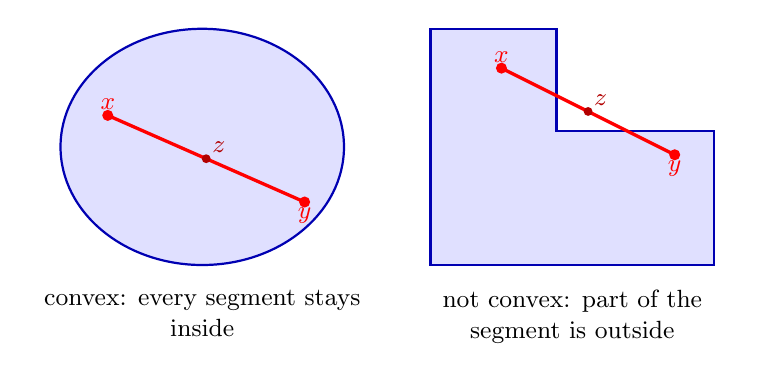
\begin{tikzpicture}[every node/.style={font=\small}]
	\begin{scope}
        % Convex model: E={(u,v): (u/1.8)^2+(v/1.5)^2<=1}.
        \filldraw[fill=blue!12,draw=blue!70!black,thick] (0,0) ellipse (1.8 and 1.5);
        \coordinate (X) at (-1.2,0.4);
        \coordinate (Y) at (1.3,-0.7);
        \coordinate (Z) at ($(X)!.5!(Y)$); % (X+Y)/2
        \draw[red,very thick] (X) -- (Y);
        \fill[red] (X) circle (2pt) node[above,inner sep=2pt] {$x$};
        \fill[red] (Y) circle (2pt) node[below,inner sep=2pt] {$y$};
        \fill[red!70!black] (Z) circle (1.6pt) node[above right,inner sep=2pt] {$z$};
        \node[anchor=north,align=flush center,text width=4.2cm] at (0,-1.7) {convex: every segment stays inside};
    \end{scope}
    \begin{scope}[xshift=4.7cm]
        % Nonconvex model: C=([-1.8,-.2]x[-1.5,1.5]) union ([-.2,1.8]x[-1.5,.2]).
        % X=(-.9,1),Y=(1.3,-.1) are inside; midpoint(.2,.45) is outside both rectangles.
        \filldraw[fill=blue!12,draw=blue!70!black,thick] (-1.8,-1.5) -- (1.8,-1.5) -- (1.8,.2) -- (-.2,.2) -- (-.2,1.5) -- (-1.8,1.5) -- cycle;
        \coordinate (X) at (-.9,1);
        \coordinate (Y) at (1.3,-.1);
        \coordinate (Z) at ($(X)!.5!(Y)$); % (X+Y)/2
        \draw[red,very thick] (X) -- (Y);
        \fill[red] (X) circle (2pt) node[above,inner sep=2pt] {$x$};
        \fill[red] (Y) circle (2pt) node[below,inner sep=2pt] {$y$};
        \fill[red!70!black] (Z) circle (1.6pt) node[above right,inner sep=2pt] {$z$};
        \node[anchor=north,align=flush center,text width=4.2cm] at (0,-1.7) {not convex: part of the segment is outside};
    \end{scope}
\end{tikzpicture}
\end{document}
